\cotefile{161-2}
\scanpage{37}
% archive sheet number: 36
\usetikzlibrary{shapes.geometric}

\diagram{\resizebox{\linewidth}{!}{\begin{tikzcd}[ampersand replacement=\&,row sep=small,column sep=small]
\&\text{anneau}\&\&\\
\text{anneau local}\arrow[ur]\&\&\text{anneau réduit}\arrow[ul]\&\text{\shortstack{spectre compact\\(\unsure{séparé})}}\arrow[l]\\
\text{anneau str.\ local}\arrow[u]\&\text{anneau intègre}\arrow[ur]\&\text{pseudocorps}\arrow[u]\arrow[ur]\&\\
\&\text{corps}\arrow[u]\arrow[ur]\arrow[r,dash]\&{}\&{}\arrow[ul,dash]
\end{tikzcd}}}

\[
\widetilde{R}_{\mathrm{zar}}\qquad
\left(A[T]/FA[T]\right)_{\unsure{F'_{*}|F'_{x}|F'}}
\]

\diagram{\begin{tikzcd}[ampersand replacement=\&,row sep=small]
X_i\arrow[d]\& /\& A^{n}\\
Y\&\deleted{\unsure{i}}\arrow[r,dash]\&Y\& U\arrow[ul]\\
\&F\arrow[d]\\
\&G\&{}\arrow[l]
\end{tikzcd}}

\figure{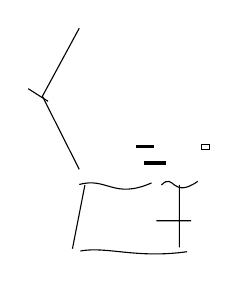
\begin{tikzpicture}[x=.36cm,y=.32cm]
\draw (-3,5.6)--(-4.3,2.9)--(-3,0); \draw (-4.8,3.2)--(-4.1,2.7);
\draw[very thick] (-1,.9)--(-.35,.9) (-.7,.25)--(.05,.25); \draw (1.3,.8) rectangle (1.58,1);
\draw (-3,-.6) .. controls (-2,-.3) and (-1.8,-1.2) .. (-.45,-.54);
\draw (-.1,-.62) .. controls (.36,-.1) and (.25,-1.2) .. (1.18,-.48);
\draw (-2.8,-.62)--(-3.24,-3.15) (.53,-.62)--(.53,-3.1) (-.28,-2.04)--(.95,-2.04) (-2.96,-3.24).. controls (-2,-3.05) and (-1,-3.55)..(.8,-3.27);
\end{tikzpicture}}

% margin note written sideways
\margin{$\forall f(a)\ \exists\unsure{e|\deleted{e}}\in\Pi(M)$ tel que $fe$ inv. et $f(1-e)$ \unsure{nilp.}}

\diagram{\resizebox{\linewidth}{!}{\begin{tikzcd}[ampersand replacement=\&,row sep=small,column sep=small]
\text{str. local}\arrow[dr]\&\&\text{\deleted{loc. intègre}}\arrow[d,dash]\\
\&\text{Spect. connexe}\arrow[d,dash]\&\text{\unsure{loc. irr.|loc. irréd.}}\arrow[d,dash]\\
\&\text{spectre irréd}\arrow[dl,dash]\arrow[dr]\&\text{\deleted{\unsure{loc. réd.}}}\&\text{\uline{réduit}}\arrow[dl]\arrow[dr]\&\&\text{spectre compact}\arrow[dl]\\
{}\&\&\text{\unsure{loc. int}}\arrow[d]\&\&\text{ps. corps}\arrow[ddl,dash]\\
\&\&\text{intègre}\arrow[dl]\&\\
\&\text{intègre normal}\arrow[d]\&\&\text{corps}\arrow[ul,dash]\\
\&\text{régulier dim $\leq$\unsure{1}}\&\&\text{(régulier dim \unsure{0})}
\end{tikzcd}}}

\diagram{\begin{tikzcd}[ampersand replacement=\&]
\Pi\arrow[d]\&[-4pt]{\subset} A\arrow[r,"{p\mapsto p^2-p}"]\& A\\
e\&[-4pt]\text{fini ?}
\end{tikzcd}}

\deleted{\unsure{anneau loc. anneau}}\quad
\deleted{\unsure{produit fini de}}\quad
\unsure{produit fini de connexes}\quad $=$ \unsure{quasi-irréductible}

\diagram{\resizebox{\linewidth}{!}{\begin{tikzcd}[ampersand replacement=\&,row sep=small,column sep=small]
{}\&\text{\uline{connexe}}\arrow[dl]\arrow[dr,dash]\&\&\text{\uline{loc$^{t.}$ irréd}}\arrow[dl]\arrow[dr]\&\&\text{\uline{réduit}}\arrow[dl,dash]\arrow[dr,Rightarrow]\&\&\text{\uline{spectre compact}}\arrow[dl]\\
\text{local}\&\&\text{\uline{irréd}}\&\text{\deleted{\unsure{quasi}}\uline{\unsure{connexe}}}\&\text{\uline{loc$^{t}$ int}}\arrow[dl,dash]\&\deleted{\unsure{corps}}\&\text{\uline{ps.-corps}}\&\\
\text{\deleted{\unsure{str local}} str. local}\arrow[u]\&\&\&\text{\uline{intègre}}\arrow[ul,dash]\&\&\text{\deleted{\unsure{quasi-}}\unsure{quasi-corps}}\arrow[ul,dash]\arrow[ur,dash]\&\\
\text{ultralocal}\arrow[u]\&\&\&\&\text{\shortstack{corps\\\deleted{\unsure{corps sép. clos}}}}\arrow[ul,dash]\arrow[ur,dash]\arrow[uuullll,dash]\\
\&\&\&\&\text{corps \deleted{\unsure{alg.}} sép. clos}\arrow[u,dash]\arrow[uuullll,dash]\&\text{\uline{\unsure{lég.es|lég$_s$}}}\\
\&\&\&\&\text{\shortstack{corps alg clos\\\deleted{\unsure{anneau}}}}\arrow[u,dash]\arrow[uuullll,dash]
\end{tikzcd}}}

\diagram{\begin{tikzcd}[ampersand replacement=\&,column sep=small]
\unsure{e|\varnothing}\arrow[r,"\sim"]\&\Pi(M)\subset A\\
e\arrow[dr,dash]\&(1-e)\arrow[d,dash]\&{}\\
\&\deleted{\unsure{A}}\&\unsure{f=}\arrow[u,dash]\\
\& f^n\& f
\end{tikzcd}}

\[
\begin{aligned}
&\forall f\quad\exists e\ \unsure{\mathrm{id}} \qquad fg=0\qquad g=f^nh\\
&A\xrightarrow{\sim}A_f\times\unsure{A/fA^{*}|A/f^{n}A}
\end{aligned}
\]

$f^n A$ \uline{stationnaire !}\qquad \deleted{$F$}

\[
 V(f)\longrightarrow V(f^n)
\]

\diagram{\begin{tikzcd}[ampersand replacement=\&,row sep=small]
\text{réduit}\arrow[dr]\&\&\text{\shortstack{loc. irréd.\\$=$ qu. irréd.}}\arrow[dl,dash]\arrow[dr,dash]\\
\&\text{\deleted{\unsure{loc.}} intègre}\&\&\text{irréd}
\end{tikzcd}}

localisations ne peut \unsure{subsister|subsérir}\qquad
mais local n'a pas \unsure{néc$^{t}$ d'alg.|d'él$^{ts}$ de} \unsure{nilpotents|nilpotence}
\deleted{\unsure{local$^{t}$ hensélien}}\quad
\uline{\unsure{demande à être|demander à être}}\quad \uline{artinien} \uline{non}

% margin note written sideways
\margin{$D_n\subset\overset{g}{\unsure{A|\mathbb A}}\times\overset{f}{A}\times\overset{e}{\unsure{A|\overline A}}$}

% margin note written sideways
\diagram{\begin{tikzcd}[ampersand replacement=\&,row sep=small]
\&D_n\arrow[d]\arrow[dl,bend right,"\unsure{p}"']\\
\deleted{\unsure{g}}\arrow[r]\&{A\times\Pi}\\
A\arrow[u,leftrightarrow,sloped,"\unsure{i}"]\&
\end{tikzcd}}

% margin note written sideways
\margin{$\unsure{e'},\ e^2=e\quad f^n(1-e)=0,\ g(1-e)=0,\ (f\mid\deleted{\unsure{\theta}}e),\ fg=e$;
\unsure{inv.} et $f^n|U_{1-e}\ \deleted{\unsure{\ne}}0$;
$\left\{\begin{aligned} f^n(1-e)&=0\\ \deleted{\unsure{f}}g(\deleted{\unsure{f}}1-e)&=0\\gf&=e\end{aligned}\right.$}

\diagram{\resizebox{\linewidth}{!}{\begin{tikzcd}[ampersand replacement=\&,row sep=small,column sep=small,cells={nodes={inner sep=1pt}}]
\&\&|[draw,ellipse]|\text{ann}\arrow[dl,dash]\arrow[d]\arrow[dr,dash]\&\&\&|[draw,rectangle]|\text{local \deleted{\unsure{artinien}}}\&\&1\\
\text{car. $p$\unsure{$^{\rm pur}$}}\&\text{\unsure{annelique}}\&\text{quasicomp}\arrow[dl]\arrow[dr,dash]\&\text{\shortstack{\unsure{annulé} par $p$\\\deleted{\unsure{divis}}}}\arrow[r,dash]\&\deleted{\unsure{alg}}\arrow[d,dash]\&\&\&1\\
\&|[draw,ellipse]|\text{connexe}\arrow[d]\arrow[dr,dash]\&\&\text{quasi-irréd}\arrow[dl]\arrow[dr]\&{}\&|[draw,ellipse]|\text{réduit}\arrow[dl]\arrow[dr,dash]\&|[draw,ellipse]|\text{compact}\arrow[d]\arrow[dr,dash]\&4\\
\&|[draw,ellipse]|\text{local}\arrow[d]\&|[draw,ellipse]|\text{irréd}\arrow[dr]\&\&\text{qu. intègre}\arrow[dl]\arrow[dr]\&\text{\unsure{localisé}}\&|[draw,ellipse]|\text{ps. corps}\arrow[dl]\arrow[dr]\&\text{\uline{\unsure{quasi-fini}}}\\
\&\text{\deleted{\unsure{local strict}}}\&\text{\deleted{\unsure{art hens.}}}\&{}\&\text{\unsure{qu. intégral}}\&{}\&{}\&1\\
\&|[draw,ellipse]|\text{str. loc}\arrow[u]\arrow[d]\&\text{\deleted{\unsure{loc hens.}}}\&|[draw,ellipse]|\text{intègre}\arrow[dr,dash]\&\&\text{qu. corps}\arrow[dl]\arrow[dr]\&\text{\unsure{pr.}}\arrow[u,dash]\&3\\
\&|[draw,ellipse]|\text{ultralocal}\arrow[drrr,dash]\&\&\text{\uline{\unsure{intégralement}}}\&|[draw,ellipse]|\text{corps}\arrow[d]\arrow[dr,dash]\&\&|[draw,ellipse]|\text{\shortstack{\unsure{non,}\\\unsure{sauf}\\\unsure{si on}\\\unsure{fixe $n$}}}\&2\\
\&\&\&\&|[draw,ellipse]|\text{corps sép. clos}\arrow[d]\&{}\&\&1\\
\&\&\&\&|[draw,ellipse]|\text{corps alg clos}\&\&\&\underline{1}\\
\&\&\&\&\&\&\&19
\end{tikzcd}}}

\[
\left\{\begin{aligned}
\text{noethériens}&\quad\text{\uline{non}}\\
\text{régulier \unsure{n.-régulier ?}}&\quad\text{\uline{non}}\\
\text{CM ?}&\quad\text{\uline{non}}\\
\text{Gor ?}&\quad\text{\uline{non}}\\
\text{int. complèt$^{e}$ ?}&\quad\text{\uline{non}}
\end{aligned}\right.
\]

\deleted{\unsure{anneau}}\quad\deleted{\unsure{propriété}}\quad
\unsure{f. f.} sur $\mathbb Z$\quad [prés. finie /$k$]

\uuline{corps parfait}\qquad
$\left\{\begin{aligned}&\text{\uline{compact parfait}}\\&=\text{\uline{pseudocorps parfait}}\end{aligned}\right.$
